% ----------------------------------------------------------------------------
% Copyright (c) 2016 by Burkhardt Renz. All rights reserved.
% Die Vorlage für eine Abschlussarbeit in der Informatik am Fachbereich
% MNI der THM ist lizenziert unter einer Creative Commons
% Namensnennung-Nicht kommerziell 4.0 International Lizenz.
%
% Id:$
% ----------------------------------------------------------------------------

\chapter{Problembeschreibung}
\label{chapter:Problembeschreibung}
In diesem Kapitel wird die Problematik, um das Generieren und Ordnen von Events in einem verteilten System mit asynchroner Kommunikation, beschrieben. Dabei betrachten man die Relevanz der Problemstellung. Ausserdem werden Fragen aufgestellt, die diese Problemstellung umfassen. Anschließend wird eine Anforderungsanalyse durchgeführt.

\section{Anwendungsüberwachung}
\label{section:Tracing von Anwendungen}
Viele Bereiche der Wirtschschaft, der Wisschenschaft und grundsätzlich des alltäglichen Lebens sind Software unterstützt. Trends wie beispielsweise \gls{iotLabel}, Hausautomatisierung, Mobile Geräte, etc. sind Anwendungsbeispiele. Diese sind aus ihrer Natur heraus stark verteilte Anwendungen. Aber auch potentiell neue Anwendungsbereiche, wie zum Beispiel verteiltes \gls{renderingGlossar}, benötigen detailierte Einsicht in die internen Vorgänge der Anwendung. 

Dabei spielen zwei Eigenschaften in der Überwachung der Anwendung eine zentrale Rolle. 
Zum einen ist das die (\lowroman{1}) \emph{Performance} und zum anderen die (\lowroman{2}) \emph{Korrektheit}.


\textbf{Performance} \space\space\space 
Viele Anwendungsbereiche setzten gewisse Rahmenbedingungen, die erfüllt werden müssen. 
Nutzererwartungen im Bezug auf interaktive Systeme, welches einer der beiden Anwendungsfälle der Instrumentalisierungsbibliothek ist, äußern sich beispielsweise in der Reaktionszeit der Anwendung auf Benutzereingaben. 
Das Rendering nimmt dabei nur einen Teil der Gesamtlatenz ein.
Ein beispielhafter Gesamtpfad, der durch die verteilte Renderinganwendung genommen werden kann, besteht aus dem Senden der Benutzereingabe, der Übermittlung der Benutzereingabe zum verteilten System, der Verarbeitung der Eingabe und der Übermittlung des Ergebnisses an die Benutzeranwendung.
\cref{fig:Anwendungsueberwachung_Gesamtsystem} verdeutlicht diesen Pfad von kausal relatierenden Events.
Dabei ist jede Komponente des Pfades ein generiertes Event.
Zu sehen ist, dass das (1) Senden der Benutzereingabe vor dem (2) Übermitteln der Benutzereingabe stattfinden.
Anschließend wird die Eingabe (3) Empfangen.
Auch die (4) Verarbeitung im verteilten System, das für den Benutzer, wie in \cref{subsection:Eigenschaften eines verteilten Systems} definiert, nicht als solches kenntlich sein muss, generiert in diesem Beispiel ein Event.
Die Antwort wird (5) gesendet und die (6) Übermittlung wird durchgeführt.
Zuletzt wird die Antwort (7) empfangen. Das Empfangen schließt den Pfad ab. Die Gesamtdauer des Pfades wird als Latenz eines Frames bezeichnet.
Daraus kann eine Durschschnittslatenz über eine Zeitspanne berechnet werden, welches als Performanceindikator dient. Die Zeitspanne zwischen den einzelnen Events können verglichen werden. Dabei ist es möglich sog. \emph{Bottlenecks} zu identifizieren. Bottlnecks sind Vorgänge, die einen großteil der Gesamtdauer ausmachen. Sind werden durch die Zeitspanne zwischen zwei Events, die auf dem \emph{kritischen Pfad} liegen, bestimmt. Diese Art der Anwendungsüberwachung soll die Möglichkeit bieten, Bottlenecks zu identifizieren. Wie in \cref{subsection:Ordnung von Events} beschrieben, verlangt eine Messung der Zeit über verschiedene physikalisch Entitäten entweder eine globale physikalische Uhr oder jeweils eine physikalische Uhr in jeder Entität, die über alle Entitäten synchrone sind beziehungsweise, synchronisiert werden. Dabei stellt sich die Frage, \emph{inwiefern eine solche Zeitmessung von Zeitspannen zwischen Events konzipiert werden kann. } 


\begin{figure}[!ht]
	\centering
	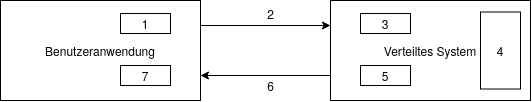
\includegraphics[scale=0.5]{img/Problembeschreibung/Anwendungsueberwachung_Gesamtsystem.png}
	\caption[Kausaler Pfad einer Vorgangs in dem verteilten rendering System]{Kausaler Pfad einer Vorgangs in dem verteilten rendering System}
	\label{fig:Anwendungsueberwachung_Gesamtsystem}
\end{figure}

\textbf{Korrektheit} \space\space\space Die Korrektheit eines Systems ist dann gegeben, wenn die Eigenschaften eines Systems einer \emph{Spezifikation} entsprechen. Das bedeutet, dass die Beobachtung des Verhaltens einer (verteilten) Anwendung nicht ausreicht, um seine Korrektheit zu beweisen. Tracing soll also nicht die Korrektheit einer verteilten Anwendung beweisen. Tracing kann aber dabei unterstützen, indem es das Verhalten einer Anwendung beobachtbar macht. Insbesondere die Zusammenhänge der Komponenten und die entstehenden Nebenläufigkeiten sind erschwerende Faktoren in der Verifikation. So stellt sich die Frage, ob \emph{kausal zusammenhängende Events derart dargestellt werden können, dass anhand einer Visualisierung feststellbar ist, ob das Verhalten der Anwendung starke Ausreißer, die auf Fehlimplmenentierung deuten könnten, aufweist.}


\section{Zusammenführung von Events}
\label{section: Ordnungsproblem von Events}
\begin{figure}[!ht]
	\centering
	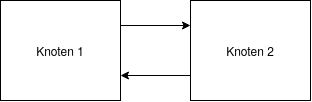
\includegraphics[scale=0.5]{img/Problembeschreibung/distributed_system_application_minimal.png}
	\caption[Minimale Struktur eines verteilten Systems]{Minimale Struktur eines verteilten Systems, bestehend aus zwei Komponenten}
	\label{fig:distributed_system_application_minimal}
\end{figure}
\begin{figure}[!ht]
	\centering
	\begin{subfigure}[t]{.49\linewidth}
		\centering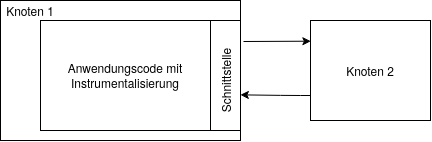
\includegraphics[width=0.9\linewidth]{img/Problembeschreibung/distributed_system_application_inside.png}
		\caption[Abbildung]{zeigt Knoten mit instrumentalisiertem Anwendungscode}
		\label{fig:distributed_system_application_inside}
	\end{subfigure}
	\begin{subfigure}[t]{.49\linewidth}
		\centering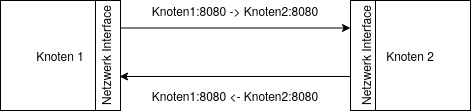
\includegraphics[width=\linewidth]{img/Problembeschreibung/distributed_system_network.png}
		\caption[Abbildung]{Netzwerkkommunikation über TCP/IP}
		\label{fig:distributed_system_network}
	\end{subfigure}
	\caption[Anwendungsinstrumentalisierung und Netzwerkkommunikation über TCP/IP in verteilten Systemen]{}
\end{figure} 

Man definieren ein minimales verteiltes System, welches das verteilte rendering System vereinfacht darstellt. Dieses besteht aus zwei Komponenten. \cref{fig:distributed_system_application_minimal} bildet ein solches System ab. Die Knoten beinhalten zwei für das Generieren und Ordnen von Events interessante Aspekte. Dies ist zum einen die in \cref{fig:distributed_system_application_inside} dargestellte verteilte Anwendung mit ihrem instrumentalisiertem Code und zum anderen das in \cref{fig:distributed_system_network} dargestellte Netzwerk, über welches Nachrichten ausgetauscht werden. 

 \begin{figure}[!ht]
	\centering
	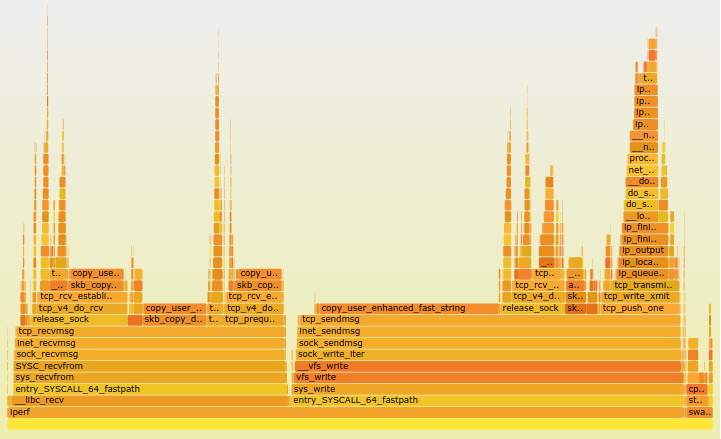
\includegraphics[scale=0.5]{img/Problembeschreibung/problembeschreibung_flamengraph.png}
	\caption[Visualisierung von CPU Performancedaten]{Visualisierung von CPU Performancedaten dargestellt als Flammengraph von Brendan D. Gregg \cite{BrendanGregg2011}}
	\label{fig:problembeschreibung_flamengraph}
\end{figure}

Die Komponenten des Systems besitzen jeweils einen Linux Kernel. Der Kernel bietet die Funktionalität \emph{perf\_events} zu erheben. 
\begin{quote}
	perf\_events ist ein eventorientiertes Überwachungswerkzeug, welches helfen kann, Leistung zu verbessern und Fehelerquellen von Funktionen zu lokalisieren. 
	\footpartcite{BrendanGreggPerf}
\end{quote}
Von dem Szenario ausgehend, dass man Events innerhalb des Minimalbeispiels analysieren möchte, eignen sich Flammengraphen.
 Der in \cref{fig:problembeschreibung_flamengraph} gezeigte Flammengraphe stellt perf\_events dar, die während einer TCP Kommunikation erhoben worden sind.  Dabei ist die Länge der Balken, die Zeit, die das Event, relativ zur Gesamtzeit der Messung, insgesamt eingenommen hat. Die erhobenen perf\_event Daten sind Stichproben. Man geht in diesem Beispiel allerdings davon aus, das alle Events aufgenommen worden sind. Diese Darstellung erlaubt es, die Events \emph{eines} Systems genau zu beschreiben. Nun kommt das zweite System hinzu, mit dem die Kommunikation stattgefunden hat. Auch hier sei gegeben, dass das zweite System Daten generiert hat, welche zu einer ähnlich aufgebaute Visualisierung führt. Die beiden Flammengraphen werden miteinandener verbunden. Dies führt zu einer dreidimensionalen Darstellung von Flammengraphen, gezeigt in \cref{fig:flamegraph_3D}. Wie in einer TCP-Verbindung üblich, wird eine Kommunikationskanal aufgebaut. Über den Kanal können Nachrichten ausgetauscht werden. Anschließend wird die Verbindung mit einem Vier-Wege-Handschlag beendet. Die obersten Blöcke und ihre systemübergreifenden Verbindungslinien, dargetellt durch die gestrichelten Linien mit Pfeilrichtung, stellen die Terminierung der TCP-Verbindung dar.
 
 Der Terminierungsprozess wird genauer betrachtet. \cref{fig:flamegraph_3D_closing} zeigt vier Events. \textbf{A} ist die \emph{FIN} Markierung des Initiators. Sie leitet die Terminierung ein. \textbf{C} stellt das Empfangen und Beantworten mittels \emph{ACK} und \emph{FIN} dar. \\
 \textbf{B} ist der Terminierungsmoment des Initatorsystems. Dieser findet nach dem Zeitpunkt des Eintreffens von \emph{FIN} des Empfänger statt. Dieser Zeitpunkt ist das Senden des letzten \emph{ACK} des Initators, addiert mit einer Konstante \emph{Timeout}.  Event \textbf{B} ist also definiert als:
 
\[
	\text{B}: \; Ack_{init} + Timeout  
\]

 \textbf{D} ist der Terminierungsmoment des Empfängersystems. Dieser Zeitpunkt ist das Erhalten der letzten, vom Initiatorsystem gesendeten, \emph{ACK} Makierung. Die unbekannte Variable \emph{Übertragungszeit} nimmt Einfluss auf den Zeitpunkt. Event \textbf{D} ist also definiert als:
 \[
 \text{D}: \; Ack_{init} + Übertragungszeit 
 \]
 
 Zu untersuchen sind die Relationen zwischen diesen vier Events.
 Dabei sind zwei Relationen, wie in \cref{subsection:Ordnung von Events} beschrieben, als $\text{A}\rightarrow\text{B}$ und $\text{C}\rightarrow\text{D}$ definiert. Durch die kausale Abhängigkeit von $\text{C}$ von $\text{A}$ gilt $\text{A}\rightarrow\text{C}$. Durch die \emph{Transitivität} ist entsprechend  $\text{A}\rightarrow\text{D}$ gegeben.  Es ist zu untersuchen, ob $\text{B}\rightarrow\text{D}$ gilt.
 Dabei sind die Bedingungen, die von Lamport definiert worden sind, zu betrachten. Da man zwei miteinander kommunizierende Systeme betrachtet, muss folgende Bedingung erfüllt sein, sodass eine \emph{Happens-Before} Relation gegeben ist. 
 \begin{quote}
 	(\lowroman{1}) Wenn $\text{a}$ das Senden einer Nachricht ist und $\text{b}$ das Empfangen derselben Nachricht in einem anderen System ist, dann $\text{a}\rightarrow\text{b}$\footpartcite{lamport78}
 \end{quote}

Nach der Definition von \textbf{D} ist es mit $\text{b}$ gleichzusetzen, somit ist ein Teil der Bedingung erfüllt. \textbf{B} ist jedoch nicht das Senden der Nachricht, also des letzten \emph{Ack}, sonder ein Event, welches darauf folgt. Die Events sind nebenläufig. Führ die TCP-Kommunikation ist dieser spezielle Zeitpunkt $\text{B}$ nicht relevant. Die Zustandsdefinitionen des TCP erlauben eine fehlerfreie Terminierung. Allerdings könnte dieser Zeitpunkt ein Anwendungsfall für Tracing sein und eine eigene Terminierung für eine ähnliche Situation benötigen. Es ist zu untersuchen, ob Events, ähnlich wie TCP Pakete, die über mehrere Tracer verteilt sein können, durch einen Terminierungsprozess eines Traces allesamt erfasst werden können.

Aus dieser Darstellung folgern zwei Fragestellungen:
\begin{quote}
	(\lowroman{1}) Müssen Traceingwerkzeuge ähnliche Terminierungsmechanismen implementieren, wie z.B Netzwerkprotokolle, um alle Events, in allen Prozessen, zu erkennen?
	
	(\lowroman{2}) Sind 3D Flammengraphen eine mögliche Darstellungsform von Tracingdaten?
\end{quote}



 

\begin{figure}[!ht]
	\centering
	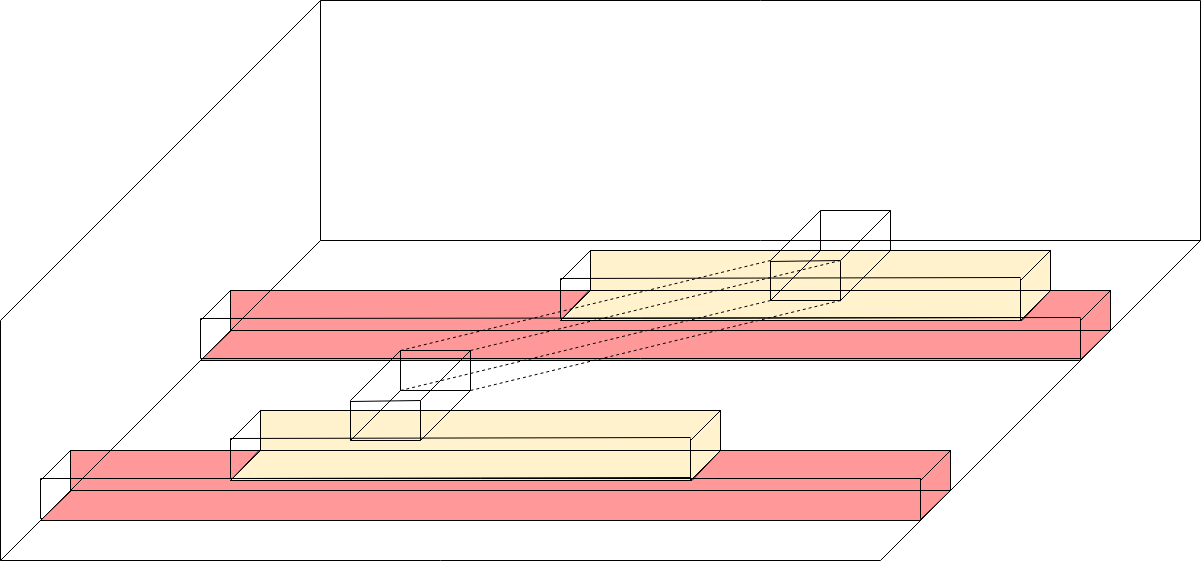
\includegraphics[scale=0.3]{img/Problembeschreibung/flamegraph_3D.png}
	\caption[3D Flammengraph]{Skizzierung eines dreidimensionalen Flammengraphs mit Nachrichtenaustausch}
	\label{fig:flamegraph_3D}
\end{figure}

\begin{figure}[!ht]
	\centering
	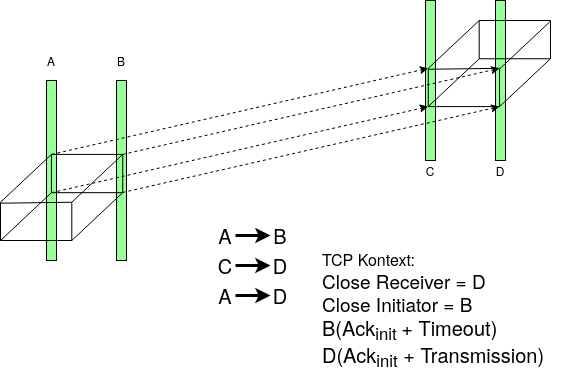
\includegraphics[scale=0.5]{img/Problembeschreibung/flamegraph_3D_closing.png}
	\caption[Flammengraph TCP schließung]{Detailierte Betrachtung des in \cref{fig:flamegraph_3D} gezeigte Nachrichtenaustauschs. Stellt die Schließung einer TCP Verbindung dar}
	\label{fig:flamegraph_3D_closing}
\end{figure}

\section{Kontextproblem von Events}
\label{section: Kontextproblem von Events}

\section{Anforderungsanalyse}
\label{section:Anforderungsanalyse}

Das Systems, für das die Instrumentalisierungsbilbiothek entwickelt wird, ist ein System für verteiltes Rendering. Die Instrumentalisierungsbilbiothek muss notwendige Funktionalitäten spezifizieren, die es ermöglichen ein Modell aus kausal abhängigen Events darzustellen. Zur Erstellung des Modells muss sich mit den Funktionalitäten der \textbf{Eventgenerierung}, der \textbf{Eventrelation}, der \textbf{Synchronisation von Eventgeneratoren}, der \textbf{Eventübermittlnug} und der \textbf{Ordnung von Events} beschäftigt werden. Im Fokus der Interpretation des Modells soll die \textbf{end-zu-end Latenz}, sowie die \textbf{Generierungszeit eines Frames} stehen. Rahmenbedingungen wie die eingeschränkte \textbf{Nachrichtenmodifikation} sind zu berücksichtigen.

Semantisch relevante Ereignisse sind zu definieren. Eine Funktionalität muss geschaffen werden, die es erlaubt, diese Ereginisse als ein Event abzubilden. Die Generierungfunktionalität muss dafür sorgen, dass die Events einem spezifizierten Aufbau aufweisen, um weiterverarbeitet und ausgewertet werden zu können. Die Nutzung einer standarisierten und erprobten \gls{apiLabel} ist wünschenswert.
 
\subsection{Funktionalitäten}

\subsubsection{Eventgenerierung}
\label{section:Eventgenerierung}
Events müssen in einem für die Anwendung semantisch relevanten Bereich generiert werden können. 

\subsubsection{Eventrelation}
\label{subsection:Eventkorrelation}
Es muss ein Modell für Events konzipiert werden. Das Modell muss in der Lage sein, Relationen abbilden zu können. Diese Relationen sollen die kausalen Zusammenhänge der Events darstellen. 

\subsubsection{Synchronistion von Eventgeneratoren}
\label{subsection:Synchronistion von Eventgeneratoren}
Eventgeneratoren sind oftmals auf verschiedenen Komponenten des verteilten Systems angesiedelt. Wie kann also ein Konzept aussehen, dass dafür sorgt, dass Events geordnet werden können.

\subsubsection{Eventübermittlung}
\label{section:Eventübermittlung}
Damit ein Kausalpfad erstellt werden kann, müssen die verstreuten Events in einer Form zusammengeführt werden können.

\subsubsection{Eventordnung}

\subsection{Interpretation des Modells}

\subsubsection{end-zu-end Latenz}

\subsubsection{Generierungszeit eines Frames}
Die Renderinggeschwindigkeit wird anhand der Zeit gemessen, also wieviele \emph{ms} gebraucht werden, um ein Bild zu generieren. gemessen Der Generierungsprozess eines \emph{Frames} umfasst vier Ebenen. Diese Ebenen sind die Applikationsebene, die Geometrieprozessierung, die Rasterung und die Pixelprozessierung. Die Verarbeitung wird, abhängig von der bearbeitet Ebene, von der \gls{cpuLabel} oder der \gls{gpuLabel} durchgeführt. Es ist wünschenswert GPU und CPU Aktivitäten überwachen zu können.

\subsubsection{Nachrichtenmodifikation}

Die Generierung von Events kann von zwei Perspektiven aus betrachtet werden.
Zum einen die \emph{Blackbox} Perspektive und zum anderen die \emph{Whitebox} Perspektive.

Bei dem Blackboxansatz, wird die Generierung angestoßen, sobald Schnittstellen angesprochen werden. Dabei werden betriebssystemspezifische Funktionalitäten genutzt, um diese Betriebssystemereignisse zu erkennen. Diese Ereginisse können erkannt, aufgearbeitet und als Events gespeichert werden. Betriebssystemspezifische Ereignisse sind vorallem ausgehende und eingehende Nachrichten, die von den Netzwerkschnittstellen verarbeitet werden. \cref{fig:distributed_system_network} zeigt eine auf dem TCP/IP Stack basierende Nachricht. Die Daten der Senderadresse, der Empfängeradresse und einem Zeitstempel könnten genutzt werden. Allerdings ist das Fehlen von Applikationsinformationen ein entscheidendes Problem. Das Ziel des Blackboxansatz ist die minimale Vorraussetzung von \emph{a priori} Informationenen über Kommunikationswege, über den Aufbau von Applikationsnachrichten, die Semantik der Anwendung und den Aufbau des verteilten Systems.\footpartcite{Aguilera2003}. Allerdings sind diese Daten äußert wichtig, um ein tiefgreifendes Verstädnis des verteilten Systems zu gewinnen. 

Der Whiteboxansatz nutzt Instrumentalisierung des Quellcodes, um die Eventgeneriernug anzustoßen. Dabei wird vorausgesetzt, dass die Semantik der Anwendung, Informationen über den Aufbau von Nachrichten, den Aufbau des Systems und die Kommunikationswege zwischen Komponenten bekannt sind. Bei der Notwendigkeit einer Modifizierung von Nachrichten weist dieser Ansatz jedoch auch schwächen auf. Im Anwendungsfall des verteilten rendering Systems fehlt die Möglichkeit, Nachrichten, innerhalb der Anwendung, um Tracingdaten zu erweitern.


% ----------------------------------------------------------------------------
